\subsection{Une intégrale fonctionnelle ?}
{
    \question{Quand notre objet est une fonction, qu'est ce que l'on entend par loi ? Comment définir l'espérance ? Peut-on intégrer selon une mesure dont la variable est une fonction ?}

    En voilà bien des questions qui semblent délicates aux premiers abords. Et-ce parceque l'on doit en effet se montrer précautionneux avec ce que l'on manipule. Les données fonctionnelles sont définies comme des variables aléatoires à valeurs dans un espace de fonction qui est en fait structuré comme un espace de Banach. Cet espace est d'autant plus effrayant qu'il est de dimension infinie.

    \begin{definition}[Données Fonctionnelles]
        On appelle donnée fonctionnelle une application $(\mathcal F, \mathit C)$ mesurable :
        \begin{equation*}
            X : \func{(\Omega, \mathcal F, \P)}{(\mathcal C^0(I, \mathds R), \norme{\infty}{\cdot}, \mathit C, \mathds P_X)}{\omega}{x = X(\omega) : t \mapsto x(t)}
        \end{equation*}
    \end{definition}
    
    \question{Dans $(\mathcal C^0(I, \mathds R), \norme{\infty}{\cdot}, \mathit C, \mathds P_X)$, quelle est précisément la tribu $\mathit C$ ? Quelle mesure sur $\mathds P_X$ pour nous permettre d'intégrer ? L'intégrale est elle une intégrale classique (Lebesgue) ?}

    On ne peut en réalité pas utiliser l'intégrale de Lebesgue. Pourquoi ? L'intégrale de Lebesgue est définie comme un supremum pris sur des fonctions étagées à valeurs réelles positives. Hors lorsque les applications sont à valeurs dans un espace de fonctions dont la dimension est infinie, la construction proposée précédemment d'intégrale n'est pas bien définie. Il faut donc redéfinir l'intégrale dans le cadre de fonctions : et donc dans un espace de Banach. Il s'agit de l'\emph{intégrale de Böchner} :

    \idee{L'idée de l'intégrale de Böchner est de reproduire les étapes de la création de l'intégrale de Lebesgue, en définissant des fonctions simples \og équivalentes \fg\footnotemark aux fonctions étagées dans le cadre réel. Si on peut construire une suite de fonctions simples qui tendent vers la fonction que l'on souhaite intégrer au sens de la topologie induite par la norme de l'espace de Banach considéré\footnotemark. L'intégrale de Böchner de notre fonction est alors la limite des suites d'intégrales des fonctions simples qui tendent vers notre fonction.}
    \footnotetext[1]{pas au sens mathématique : dans le sens \og jouant le rôle de \fg }
    \footnotetext[2]{En réalité c'est plutôt $\int \norme {\mathds B} {f - s_n} \tend n \infty 0$. Mais l'idée est bien de regarder la convergence au sens de la norme de l'espace considéré}



    \book{
        Jeon (2020) \cite{jeon2020additive}, Park et Byeong formalisent et dérivent les propriétés de l'intégrale de Böchner de façon plus adaptée à la statistique, notamment en considérant des densités. Ils étendent désormais les résultats que l'on a exposés précédemment dans le cadre réel au cadre hilbertien (qui est un cas particulier des espaces de Banach en considérant la norme issue du produit scalaire).\cite{cho2023partially, jeon2022additive, lee2023hilbertian}
    }

    Les auteurs (Park, Byeong, Jeon, \dots) utilisent dans l'ensemble de leurs articles traitant des données hilbertiennes ou dans un espace de Böchner les notations :
    \begin{todolist}
        \item $\oplus$ : addition interne
        \item $\odot$  : multiplication externe
        \item $\ominus = \bullet \oplus [(-1) \odot \bullet ]$ : soustraction interne
    \end{todolist}

    \smallskip

    \noindent pour mettre sur l'emphase d'avoir des opérations adaptées aux données, qui ne sont pas nécessairement les lois de composition usuelles. Toutefois, dans le reste de ce document, nous n'utiliserons que la notation $\odot$ en dehors des notations usuelles pour ne pas alourdir la lecture.

    \bigskip

    \noindent Afin de mieux comprendre l'opération d'intégration avec laquelle on travaille, on peut comparer la construction de l'intégrale de Lebesgue et celle de l'intégrale de Böchner via le schéma suivant :
    
    \begin{figure}[H]
        \centering
        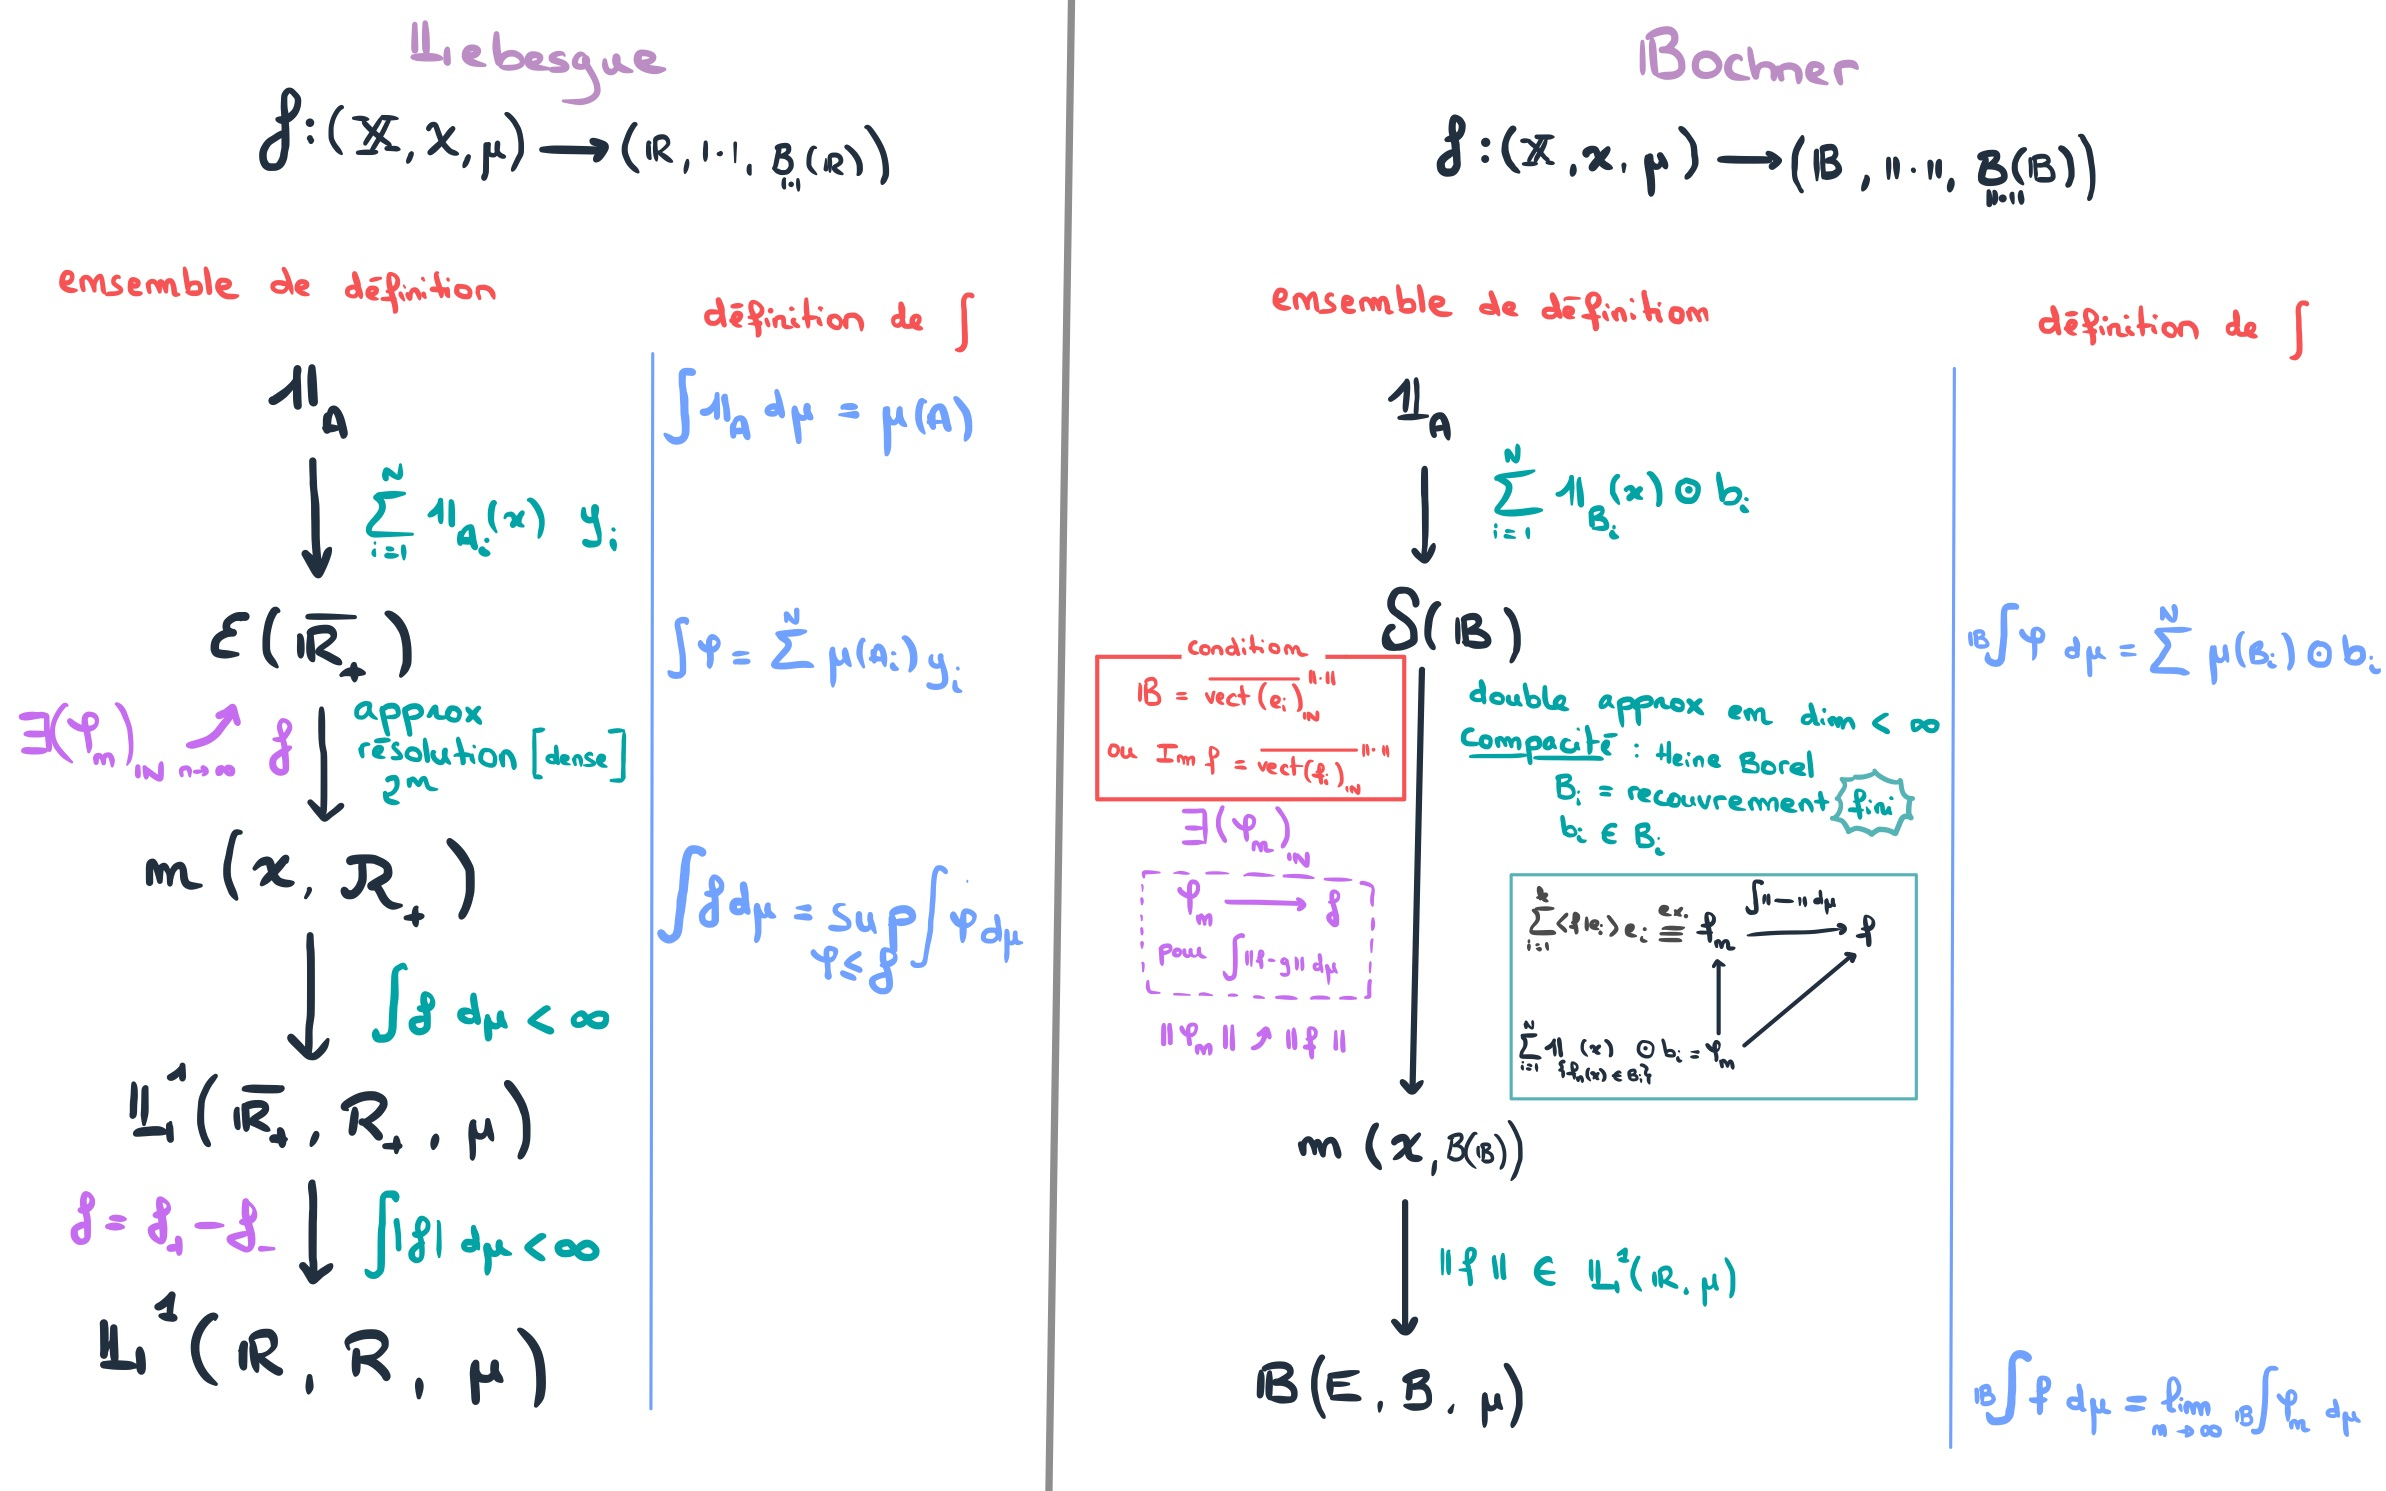
\includegraphics[width=\textwidth]{Images/bochner_vs_leb.jpeg}
        \caption{Différences entre la construction de l'intégrale de Lebesgue et la construction de l'intégrale de Böchner}
        \label{fig:boch-vs-leb}
    \end{figure}

    
    
    
}



\subsection{Existence de loi à densité}
{

    Le problème précédent a été résolu en construisant une intégrale sur des espaces vectoriels normés et en exploitant le fait que la norme est une application d'un espace vectoriel normé dans l'ensemble des réels positifs sur lequel on dispose de l'intégrale de Lebesgue. Pour étendre les travaux sur l'estimation du modèle additif lorsqu'il y a des erreurs de mesure sur les covariables on a désormais besoin de disposer de lois à densité sur nos espaces de fonction. 

    \bigskip
    
    L'intégrale de Böchner a peu été utilisée en statistiques, c'est pourquoi \cite{jeon2020additive} dérive et expose brièvement les résultats importants sur l'intégrale de Böchner pour les lois à densité, qui sont clés dans l'estimation du modèle additif par l'algorithme du Backfitting avec l'approche de Mammen (1999) \cite{mammen1999existence}, dont les auteurs suivent les pas pour l'étendre au cadre hilbertien. L'idée est de montrer qu'en supposant que $\mathds P_X \ll \mu$ et $\esperance{\lVert f(X) \rVert} < \infty$, la quantité :

    \begin{equation}
        \displaystyle\int_{\mathds B} f(x) \odot p_X(x) \, d\mu(x) = \esperance{f(X)}\label{eq:bochner_densite}
    \end{equation}

    et de même si $\mathds P_{X, Z} \ll \mu \otimes \nu$ et $\esperance{\lVert f(X) \rVert} < \infty$ alors la quantité :

    \begin{equation}
        \displaystyle\int_{\mathds B} f(x) \odot \frac{p_{X, Z}(x,z)}{p_Z(z)} \, d\mu(z) \overset{\textsf{version}}= \esperancesachant Z {f(X)}\label{eq:bochner_densite_cond}
    \end{equation}
    
    C'est alors qu'un problème majeur survient :

    \nope{\smallskip\centering Sur un espace de Banach quelconque, la propriété de Radon-Nikodym n'est pas vérifiée. Pire, elle ne peut être vérifiée par un ensemble contenant $\mathcal C^0\bigl( [0,1] \bigr)$}

    Expliquons un peu plus en détails l'insertion précédente.
    \subsubsection{Théorème de Radon-Nikodym}
    {
        Une des méthodes les plus naturelles pour créer de nouvelles mesures est de prendre une mesure que l'on connait déjà et de pondérer la répartition de la masse des objets qu'elle mesure. On appelle cela une mesure à \og densité \fg, très utilisée notamment en probabilité pour dériver de multiples \og lois continues \fg à partir de la mesure de Lebesgue particulièrement adaptée à la topologie de $\grandR$.

        \smallskip  

        \noindent On dit que la mesure $\nu$ est à densité par rapport à $\mu$ si il existe une fonction $\mu$-intégrable $\frac{d\nu}{d\mu}$ telle que :

        \begin{equation*}
            \nu : \func{\mathcal X}{\Rplus}{A}{ \leb_{\mathds X} \indicatrice{ A }(x)\frac{d\nu}{d\mu}(x) \, d\mu(x) }
        \end{equation*}

        \question{\smallskip\centering Peut-on à partir de n'importe quelle mesure déterminer une mesure à densité ?}
        
        Toute mesure\footnote{toute mesure *$\sigma$-finie*} qui ne voit pas plus de détails que la mesure d'origine\footnote{On dit que la mesure est absolument continue par rapport à la mesure d'origine, one note $\nu \ll \mu$} admet une densité par rapport à la mesure d'origine. On appelle cette densité la dérivée de Radon-Nikodym. 

        \noindent Il se trouve que cette propriété qui s'avère pratique pour construire des lois de probabilités sur $\R d$ n'est plus vraie en général pour les espaces de Banach munis de l'intégrale de Böchner. Le lecteur pourra se référer à \cite{Ryan2002} pour plus de précisions sur l'existence d'espaces de Banach qui ne disposent pas de la propriété de Radon-Nikodym.
        
        \bigskip

        \noindent Un point clé pour notre intérêt d'étendre la méthode vue précédemment au cas fonctionnel est le fait que tout espace contenant l'ensemble des fonctions continues sur $[0,1]$ ne possède pas cette propriété, ce qui nous dérange fortement étant donné que l'on travaille sur ces objets.\cite{Ryan2002} 
        
        \warn{
            Ce que l'on vient d'énoncer sur la non validité de la propriété de Radon-Nikodym des espaces de Banach munis de l'intégrale de Böchner ne stipule pas qu'il n'existe pas de loi à densité. Il nous dit juste que la proposition \og $\nu$ est absolument continue par rapport à $\mu \implies \exists \frac{d\nu}{d\mu}, \ \nu = \frac{d\nu}{d\mu} \cdot \mu$ \fg n'est pas vraie. Ce qui veut juste dire que trouver des densités devient plus compliqué.
        }

        Ainsi dans les propositions \eqref{eq:bochner_densite_cond} et \eqref{eq:bochner_densite} énoncées précedemment, je ne suis pas personnellement convaincu de l'insertion directe $\esperance{\lVert f(X) \rVert} < \infty$ et $\mathds P_X \ll \mu \implies \eqref{eq:bochner_densite}$ puisque la non validité de la propriété de Radon-Nikodym dans les espaces de Banach en général nous dit que la continuité absolue n'est pas un critère suffisant pour admettre une densité. Cependant, il se pourrait que je n'ai pas bien compris les arguments des auteurs, et que l'on puisse toujours trouver une densité à partir de l'absolue continuité en se restraignant aux espaces de fonctions qu'ils considèrent. Dans le bénéfice du doute, je remets cette question à mon incompréhension pour le moment.
        

        
        
        \subsubsection{Une construction de la théorie autour de l'estimation à noyaux compliquée}
        
        Une partie non négligeable de la théorie non paramétrique pour les données fonctionnelles a été développée en se basant sur un estimateur de Nadaraya-Watson impliquant l'étude de la probabilité dite de petite boule qui étudie à quel point deux observations sont proches dans l'espace (ce qui relève évidemment d'une importance capitale pour un estimateur de localisation):
        
        \begin{equation}
            \proba{ d(X_a, X_b) < \varepsilon } \textsf{ lorsque } \varepsilon \rightarrow 0
        \end{equation}

        \noindent dont l'utilité est parfaitement expliquée dans \cite{selk2023nonparametric} :

        \citer{La (semi-)distance joue également un rôle important pour les propriétés asymptotiques des estimateurs fonctionnels non paramétriques. 
        %Le chapitre 13 de Ferraty et Vieu (2006) est consacré à cette question. 
        [...]
        La probabilité de petite boule définie comme $\proba{ d(u,v) < \varepsilon }$ apparaît dans le taux de convergence de nombreux estimateurs non paramétriques tels que l'estimateur fonctionnel de Nadaraya-Watson. 
        Si la probabilité de petite boule décroît très rapidement lorsque $\varepsilon$ tend vers zéro (en d'autres termes, si les données fonctionnelles sont très dispersées), la vitesse de convergence sera faible, alors qu'une probabilité de petite boule décroissant suffisamment lentement conduira à une vitesse de convergence similaire à celles trouvées dans les environnements de dimension finie.
        
        \flushright{\dash Selk, Leonie and Gertheiss, Jan (2023) \cite{selk2023nonparametric}}}

        %\citer{The (semi-)metric also plays an important role for the asymptotic properties of nonparametric functional estimators. Chapter 13 in Ferraty and Vieu (2006) is dedicated to this issue. The small ball probability that is defined as $\proba{ d(u,v) < \varepsilon }$ appears in the rate of convergence of many nonparametric estimators such as the functional Nadaraya-Watson estimator. If the small ball probability decays very fast when $\varepsilon$ tends to zero (in other words, if the functional data are very dispersed) the rate of convergence will be poor, whereas a small ball probability decaying adequately slowly will lead to a rate of convergence similar to those found in finite dimensional settings.}

        Il faut faire d'autant plus attention lorsque l'on travaille avec les probabilités de petites boules dans des espaces fonctionnels comme $\mathcal C⁰ \bigl( [0,1] \bigr)$ qui est de dimension infinie :

        \warn{
        il a été démontré qu'une hypothèse qui était fréquemment utilisée par certains auteurs en estimation non paramétrique fonctionnelle concernant les probabilités de petites boules implique que l'espace de fonction considéré est de dimension finie. \cite{azais2013remark} Cela restreint fortement la flexibilité qu'offrent les données fonctionnelles.
        }

        \noindent Cela illustre bien un point fondamental lorsque l'on travaille avec les objets fonctionnels :

        \begin{todolist}
            \item Les espaces de fonctions généraux sont de dimension infinie
            \item[\crossed] Les espaces de dimension infinie sont \textbf{hautement contre-intuitifs} et difficiles à manipuler
            \item En statistique, on travaille avec des hypothèses sur le comportement des observations : on doit faire attention aux hypothèses que l'on pose sur les objets fonctionnels qui pourraient restreindre leur flexibilité
            \item[\checked] Travailler avec des sous-espaces de dimension finie n'est pas pour autant inutile, les fonctions polynômiales de degré $d$ sont de dimension finie et s'avèrent être très utiles dans un nombre important de problèmes
            \item[\crossed] Il semble toutefois judicieux de développer une théorie générale sur les données fonctionnelles qui s'appliquerait à la plus gande variété de fonctions possible (et donc de dimension infinie), et on doit bien vérifier sur quoi travaille chaque résultat statistique 
            
        \end{todolist}


        \subsubsection{Définir une densité sur les données fonctionnelles}
        
        Pouvoir définir une mesure à densité sur les données fonctionnelles s'avère de plus en plus critique au fur et à mesure que de la théorie sur l'estimation non paramétrique basé sur de telles données voit le jour.
        Une extension naturelle de l'estimateur de Nadaraya-Watson aux données fonctionnelles est :

        \begin{equation}
            \widehat m : \func{\mathcal C^0\bigl(I, \mathds R\bigr)}{\mathds R}{x}{
                \displaystyle\frac{\sum_i Y_i \cdot K\left( \frac{d(x, X_i)}{h} \right)}{\sum_i K\left( \frac{d(x, X_i)}{h} \right)}
            } \textsf{ où } d \textsf{ est une semi-distance sur } \mathcal C^0(I, \mathds R)
        \end{equation}

        % TODO : refaire
        P. Hall et A. Delaigle (2010) commencent par reconnaître que, comme nous l'avons vu précédemment, dans le cadre des données fonctionnelles la densité n'est en général pas bien définie. Ils proposent alors de définir une \og densité \fg sur un espace fonctionnel à une résolution spécifique qui correspond à un nombre composantes principales à sélectionner dans l'approximation de notre donnée fonctionnelle : cela nous permet de nous ramener à de la dimension finie. Enfin le concept de densité serait lié à la densité des scores\footnote{les scores sont les composantes de la fonction aléatoire centrée sur la base ACP $\suite \psi k$ : $\prodscalselon {X - \esperance X} {\psi_k} {\mathds L^2}$. Ce sont des variables aléatoires réelles.} dans la base ACP tronquée des données fonctionnelles étudiées, ce qui nous avantage puisque l'on sait bien mieux manipuler les densités dans le cadre des variables aléatoires réelles.\cite{delaigle2010defining} La particularité de pouvoir utiliser cette approche même lorsqu'une densité "hilbertienne" n'existe pas rend cette approche attractive. Les auteurs considèrent une log-densité des scores qui représente le comportement à l'ordre 1 de l'effet de la valeurs des scores sur les probabilités que deux fonctions soient proches (probabilité de petite boule).

        \bigskip

        Soient $(\xi_k)_{\mathds N}$ les scores de la fonction aléatoire $X$ dans la base ACP $\suite \psi k$ et $r(h)$ le nombre de composantes principales à considérer pour l'approximation de $X$ à la résolution $h$. On note $\xi = \famfinie[k] \xi 1 {r(h)}$ et $e = \famfinie[k] e 1 {r(h)}$ une réalisation de $\xi$. On définit alors la log-densité des scores comme :

        \begin{equation}
            \ell(e | h) = \frac 1 {r(h)}\sum_{k=1}^{r(h)} \log p_{\xi_k} (e_k)
        \end{equation}

        Alors à condition que les scores $\xi_k$ soient i.i.d et que les $|p_{\xi_k}^{''}| < \infty$ sans s'annuler\footnote{c'est un cas particulier des conditions plus générales mentionnées dans \cite{delaigle2010defining}, ce qui allège la lecture}, la probabilité de petite boule à la résolution $h$ est :

        \begin{equation}
            p(e | h) = \proba{ \sum_{k=1}^\infty \lambda_k (\xi_k - e_k)^2 \leq h^2 } =\widetilde C \cdot e^{r(h)\ell(e | h) + o\bigl(r(h)\bigr)}
        \end{equation}
        
        \chk{La \og densité \fg ainsi définie permet de travailler sur les scores des données fonctionnelles, et de donner des informations sur les probabilités de petite boule, ce qui est un point clé pour l'estimation non paramétrique. De plus cette définition de densité se base sur les scores des données fonctionnelles, objets importants et spécifique de ces dernières, ce qui motive d'avantage cette approche. }
    }
}
